A sparse grid that is fully nested and, moreover, well disposed to adaptivity,
as we shall see, can be constructed using the (one-dimensional) Newton--Cotes
rule \cite{ma2009}. For each level, the rule is merely a set of equidistant
nodes on $[0, 1]$.

\begin{remark}
Equidistant nodes are known to perform poorly when interpolating with
polynomials of high orders (Runge's phenomenon). However, it is not a concern
for us as our basis functions are of lower orders, as discussed in
\sref{basis-functions}.
\end{remark}

The rule comes in two flavors: closed and open. The only difference between the
two is that the former includes the endpoints, that is, 0 and 1, while the
latter does not. Now, in \sref{smolyak-algorithm}, we postulated that the
assumption in \eref{tensor-exactness} was needed to proceed. The closed rule
satisfies this assumption, and it is the one used in the original version of
local adaptivity presented in \cite{ma2009}. The open Newton--Cotes rule, on the
other hand, violates the assumption close to the boundaries of the interval.
However, we found that the open rule is a viable option since it performs well
in practice, which was also noted in \cite{klimke2006}. In fact, we were able to
obtain better results with the open rule and decided to advocate for it in the
paper.

\begin{figure}[t]
  \centering
  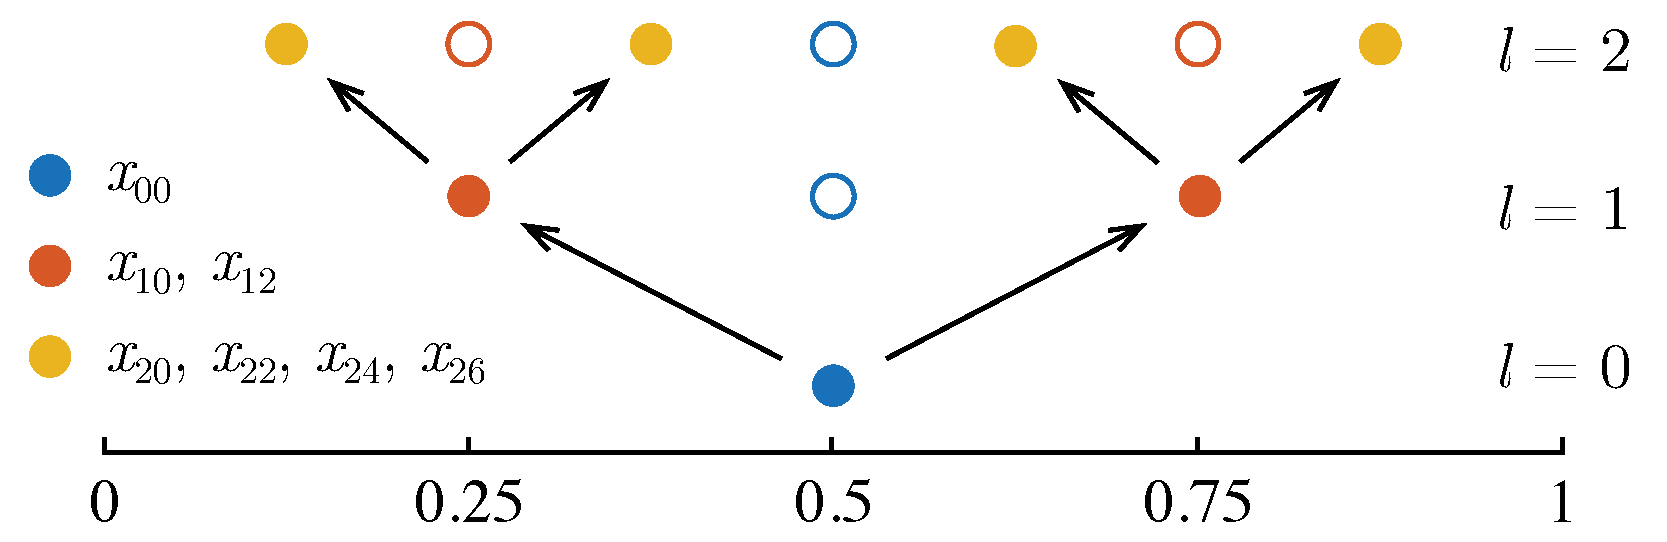
\includegraphics[width=1.0\columnwidth]{include/assets/figures/grid.pdf}
  \vspace{-1.5em}
  \caption{
    The open Newton--Cotes rule for the first three level of one-dimensional
    hierarchical interpolation.
  }
  \flab{grid}
\end{figure}

The open Newton--Cotes rule of level $i \geq 0$ is
\begin{equation} \elab{newton-cotes-grid}
  \X_i = \left\{ x_{ij} = \frac{j + 1}{\n_i + 1} \right\}_{j \in \oindex_i}
\end{equation}
where $\oindex_i = \left\{ i - 1 \right\}_{i = 1}^{\n_i}$ and $\n_i = 2^{i + 1}
- 1$. The first three levels of the rule are depicted in \fref{grid}. It can be
seen that the number of nodes (in one dimension) grows as 1, 3, 7, 15, 31, and
so on, and that the rule is fully nested. In multiple dimensions, the nodes are
formed as shown in \eref{collocation-nodes}.
